\cotefile{162-5}
\scanpage{42}
qu'i\unsure{\deleted{o}l} conviendra de poser les définitions adéquates). - Peut-être Quillen\linebreak
\margin{\uuline{oui}} \margin{\figure{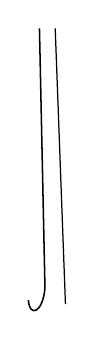
\begin{tikzpicture}[x=1cm,y=1cm]\draw[line width=.55pt] (0,3.5) -- (.07,.20) .. controls (.04,-.12) and (-.13,-.17) .. (-.14,.05);\draw[line width=.45pt] (.20,3.5) -- (.33,0);\end{tikzpicture}}}a-t-il une définition semi-si\unsure{\deleted{p}m}pliciale plus directe, sans passer par des\linebreak
n-catégories, des $K_i$ et plus précisément du H-espace qui devrait correspon-\linebreak
dre à C. \deleted{Dans le cas} Ce n'est certainement pas \inserted{en général} l'ensemble semi-simplicial\linebreak
SC \deleted{engendré à} associé à C, puisque dans le cas d'une catégorie additive,\linebreak
C est homotopiquement trivial (en effet le foncteur identique est ``homotope\linebreak
au foncteur nul, puisqu'il suffit d'avoir un homomorphisme d'un foncteur\linebreak
dans l'autre; d'où une équivalence d'homotopie entre C et la catégorie\linebreak
nulle). Pourtant, il semble bien que dans le cas où C est une Gr-catégorie\linebreak
\margin{\unsure{$\xi$|$\zeta$}} \margin{\figure{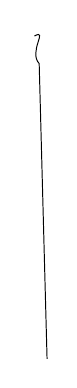
\begin{tikzpicture}[x=1cm,y=1cm]\draw[line width=.35pt] (0,4.1) .. controls (.18,4.2) and (-.08,3.9) .. (.06,3.75) -- (.16,0);\end{tikzpicture}}}i.e. admet des inverses, alors ce soit bien la construction ``naïve'' SC qui\linebreak
est la bonne, puisqu'on trouve bien un $\pi_o$ et un $\pi_1$ qui sont aussi les\linebreak
$\pi_o$ et $\pi_1$ au sens catégorie sans Gr-structure.

\margin{À expliquer : pour des Gr-n-catégories, les $\pi_i$ au sens\linebreak
\unsure{$\xi$|$\zeta$} \figure{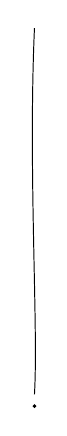
\begin{tikzpicture}[x=1cm,y=1cm]\draw[line width=.35pt] (0,4.8) .. controls (-.08,3) and (.05,1) .. (0,.15);\fill (0,0) circle (.025);\end{tikzpicture}} semi-simplicial sont aussi les $\pi_i$ au sens Gr-n-catégories,\linebreak
savoir les objets à isom près dans divers $\underline{\mathrm{Hom}}(1,1)$ ...... \deleted{Il y a\linebreak
aussi une interprétation de l'opération \unsure{$\Omega$ : espace des lacets}\linebreak
en termes d'opération \unsure{du|de} shift géométrique évidente sur les\linebreak
n-catégories .....}}

\margin{41}
